\documentclass{article}

\usepackage{amsmath}
\usepackage{gensymb}
\usepackage{graphicx}
\usepackage{caption}

\title{On the Properties of Solenoid Originated Magnetic Fields} % Sets article title
\author{Elliott Ashby}
\date{\today}


\begin{document}
    \maketitle
    
    \section{Introduction}
    
    \subsection{Aim}
    This small project aims to investigate some of the properties of 
    solenoid originated magnetic fields. 
    \newline This will be accomplished with a combination of theoretical 
    calculations along with experimental evidence.
    \subsection{Methods}
    \subsubsection{Neutralising Magnetic Fields}
    \begin{enumerate}
        \item Zero hall monitor agaist earths magnetic fields.
        \item Position two solenoids 20cm apart. Such as in \textbf{Figure 1}.
        \item Reverse current connections on one of the solenoids in order to reverse the direction of the magnetic fields.
        \item Set power supply to 1.5A.
        \item In a systematic manner, vary the hall probe along the common axis of the the solenoids and record the magnetic field in Gauss and the distance from a solenoid of ones choice.
        \item Plot Gauss against distance z (cm).
    \end{enumerate}
   \subsubsection{Alternate Axis Measurements from a Single Solenoid}
   \begin{enumerate}
       \item Zero hall monitor agaist earths magnetic fields.
       \item Set up a single solenoid at 1.5A.
       \item Vary the hall probe's distance along the x axis 90\degree from +z\textsubscript{0} (z\textsubscript{0}=13cm for our measurements) as seen in \textbf{Figure 2}.
       \item Record hall effect in Gauss and distance x in cm.
       \item Plot Gauss against distance x (cm).
   \end{enumerate}
   \begin{figure}
       \centering
       \includegraphics[scale=0.56]{/home/tex/images/scrots/2021-12-07-00:30:10-screenshot.png}
       \caption{A Helmholtz pair}
   \end{figure}
   \begin{figure}
       \centering
       \includegraphics[scale=0.9]{/home/tex/images/scrots/2021-12-07-00:35:01-screenshot.png}
       \caption{Alternate Axis Setup}
   \end{figure}
   
   \section{Results}
   \subsection{Neutralising Magnetic Fields}
%    \begin{figure}
%        \centering
%        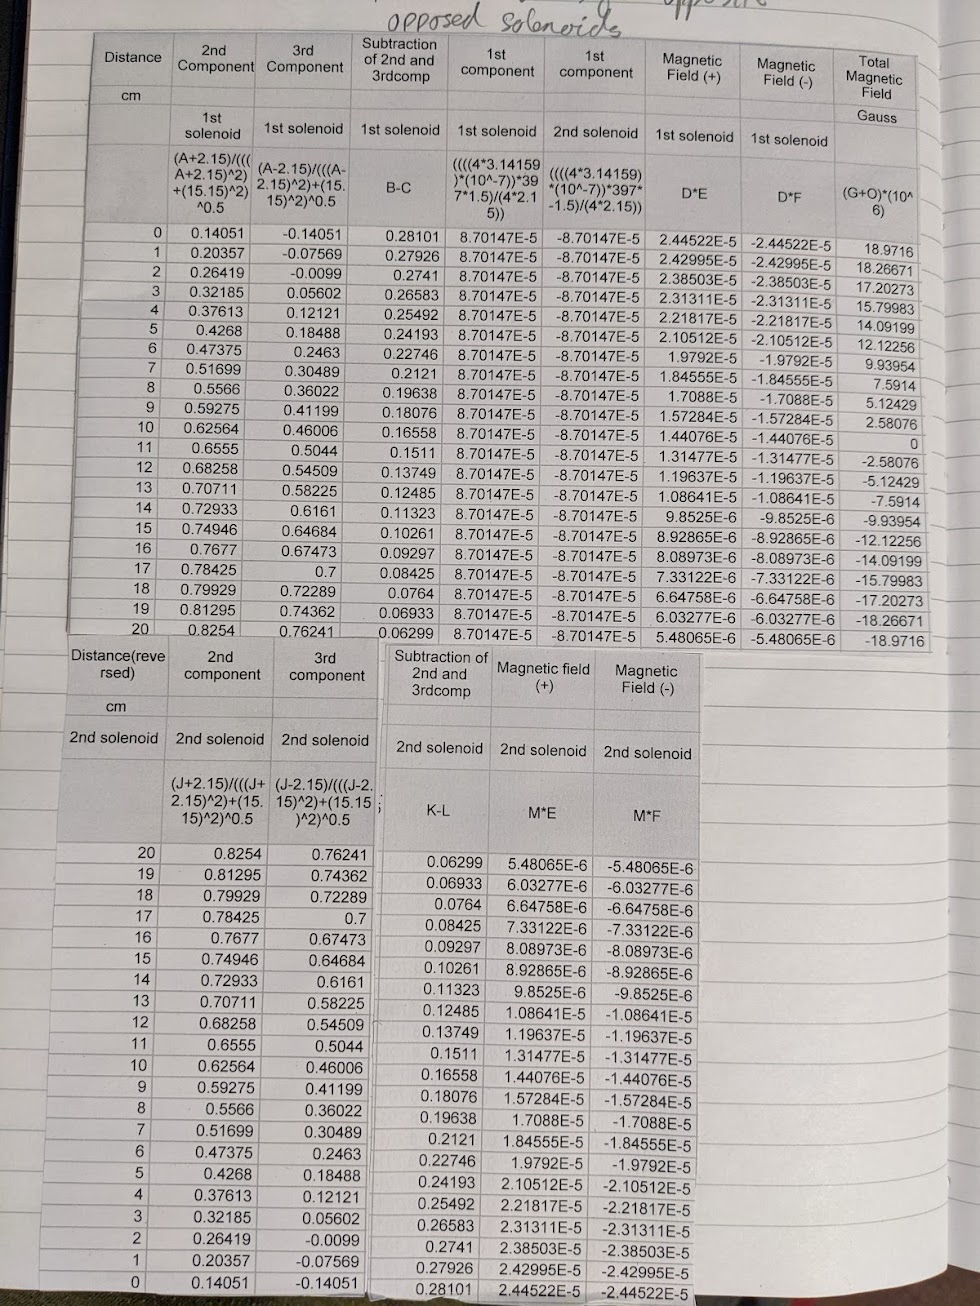
\includegraphics[scale=0.3]{/home/tex/Documents/Work/physics/latex/media/images/theorysol.jpg}
%        \caption{Theoretical Values for Neutralising Magnetic Fields}
%    \end{figure}
   \begin{figure}
       \centering
       \includegraphics[scale=0.6]{/home/tex/images/scrots/2021-12-07-00:30:45-screenshot.png}
       \caption{Graphing Theoretical Magnetic Field in Gauss against z distance in cm}
   \end{figure}
%    \begin{figure}
%        \centering
%        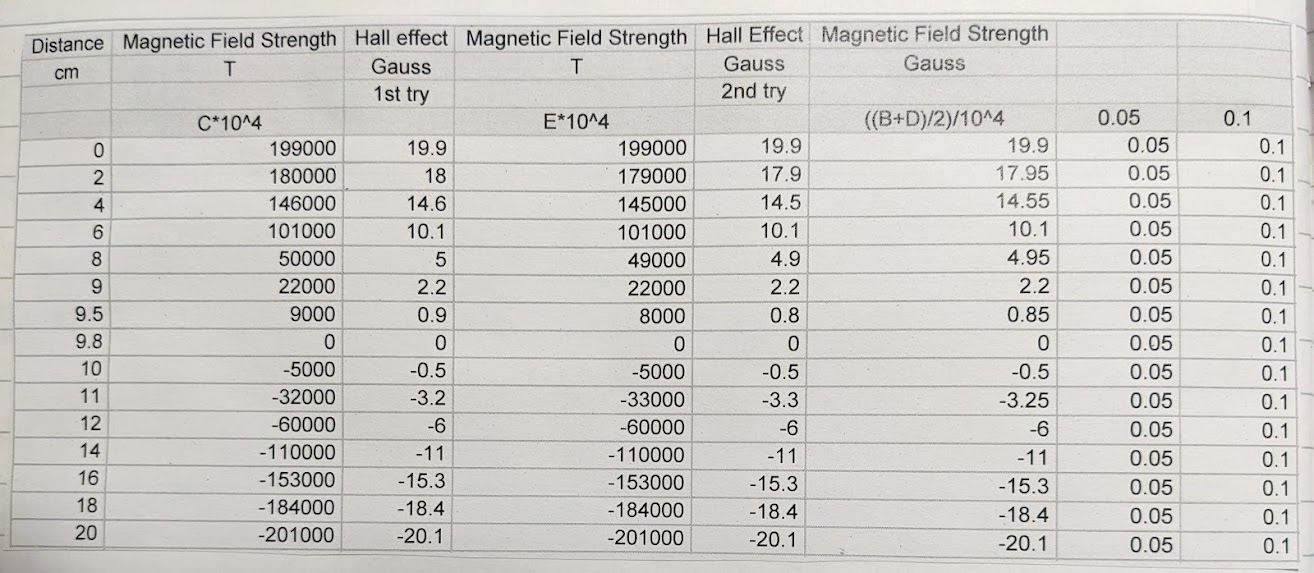
\includegraphics[scale=0.3]{/home/tex/Documents/Work/physics/latex/media/images/expres.jpg}
%        \caption{Experimental Values for Neutralising Magnetic Fields}
%    \end{figure}
   \begin{figure}
       \centering
       \includegraphics[scale=0.6]{/home/tex/images/scrots/2021-12-07-00:30:34-screenshot.png}
       \caption{Graphing Experimental Magnetic Field in Gauss against z distance in cm}
   \end{figure}
   The magnetic fields generated by the opposed solenoids can be seen in \textbf{Figure 3}
   creating a system of magnetic fields between the 2 solenoids that oppose each other. The theoretical values can be calculated
   with the \textbf{Biot-Savart Law};
   \begin{equation}
       d{\bf{B}} = \frac{{\mu _0 }}{{4\pi }}\frac{{Id\ell \times {\bf{\hat r}}}}{{r^2 }}
   \end{equation}
   \textbf{B} in (1) is measured in Tesla, so in order to compare it to our experimental values, we converted it to Gauss by
   multiplying by 10\textsuperscript{4}. \newline
   In order for a calculation to be done on a coil like those found in a Helmholtz pair in order to find magnetic field strength at 
   distance z from the centre of one of the coils, the Biot-Savart Law is derived into equation (2) where I is the current, \(\mu\)\textsubscript{0} is the permeabilty 
   constant and N are the number of loops in the solenoid.
   \begin{equation}
       B_z = \frac{\mu _0 N I}{A \ell}\bigg( \frac{z + \ell}{\sqrt{(z + \ell)^2 + R^2}} - \frac{z - \ell}{\sqrt{(z - \ell)^2 + R^2}}\bigg)
   \end{equation}
   Using known values of N = 397, I = 1.5A, A
   \subsubsection{Expected Results}
   The results expected from this experiment are as follows
   \begin{itemize}
       \item The same magnitude of magnetic field at distances 0cm and 20cm.
       \item Manetic field 0 Gauss at 10cm.
       \item Opposing quadratic relationships "added" together to create a cubic relationship since the magnetic field strength varies like \(\frac{1}{r^2}\).
   \end{itemize}
   These critical features can clearly be seen in theoretical values calculated seen graphed in \textbf{Figure 3}.
   \subsubsection{Observed Results}
   From experimental values shown in \textbf{Figure 4}, these features can clearly be identified in relation to the expected model, however, accounting
   for standard uncertainty represented in the curve fit, some aspects are still far from theoretical values. These aspects and possible explanations include;
   \begin{itemize}
       \item Different values at 0cm and 20cm \(\rightarrow\) This arises from the two solenoids generating different magnetic fields from the same current supply,
       as seen from \textbf{Figure 3}, a differance of 0.2 Gauss in magnitude can be observed, with the solenoid generating a more powerful magnetic field
       being the one located at 20cm. This may be for a variety of reasons such as different number of loops, higher density of loops or lower resistance.
       \item The experimental difference referenced above also affects a non 0 Gauss measurement at 10cm \(\rightarrow\) Due to the difference in generated magnetic fields
       and the solenoid located at 20cm being stronger at the same current of 1.5A, instead of the magnitudes of magnetic field being equal at equal radius, they are instead 
       different by 0.5 Gauss bias toward the solenoid located at 20cm. This means that the actual location of equilibrium of the magnetic fields is at 9.8cm instead of 10cm.
       \item Another inconsistency is in the absolute values when compared to theoretical values, most easily seen at 0cm and 20cm, where comparing theoretical against experimental yields 
       differences from the expected 18.97 Gauss where the solenoids at 0cm generate a magnitude of 19.9 Gauss and at 20cm generate a magnitude of 20.1 Gauss. \(\rightarrow\) If you consider 
       an average of the two experimental values at 20 Gauss, this is roughly 1 Gauss higher than the expected theoretical value. While we are unsure as to what definitively caused this difference 
       since 1 Gauss difference is much larger than the uncertainty maximum of \(\pm\)0.11 Gauss one can speculate that this difference is perhaps due to other factors such as greater unmeasurable inaccuracies
       in the hall probe or miscalculations in the hall voltage to gauss automated calculations not under our control.
   \end{itemize}
   Focusing now on the similarities;
   \begin{itemize}
       \item Experimental results yielded values and relationships extremely similar to theoretical values (\textbf{Figure 3, Figure 4}), both boast a negative cubic relationship 
       formed from the difference of two \(\frac{1}{r^2}\) relationships.
       \item The polynomial curve fits of \textbf{Figure 3} and \textbf{Figure 4} have similar coefficients, the largest difference being the coefficient of x at 0.08, however this is only 6.625\% of the average of the 
       two coefficients. Considering other inaccuracies that cannot be measured due to our setup, this is a reasonable difference of fits such that their similarity can be noted.
   \end{itemize}


\end{document}